\documentclass{article}

%\usetikzlibrary{automata,positioning}

\usepackage{graphicx}
%\usepackage{landscape}
 \usepackage{nopageno}

\usepackage{array}
\usepackage{tikz}
\begin{document}

\rotatebox{90}{
\begin{tabular}{p{240pt}|p{240pt}}
\begin{center}{\LARGE
\textbf{Logistic regression}
}\end{center} 
& 
\begin{center} 
{\LARGE
\textbf{Neural Networks}
}
\end{center}
 \\
\hline
%  \begin{center}
%  \vspace{20pt}
\vspace{30pt}
\hspace{-30pt}
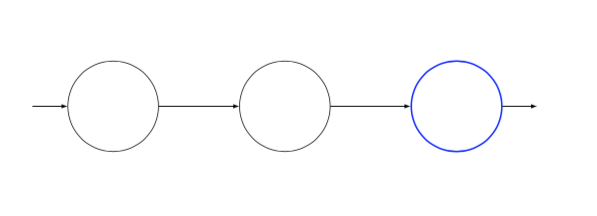
\includegraphics[scale=0.4]{logistic_color_no_expression.png}  
%\end{center}
&
\begin{center}
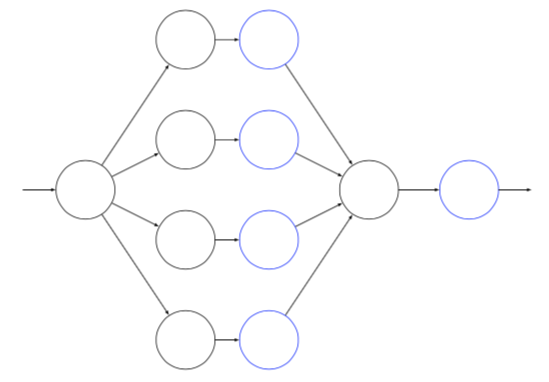
\includegraphics[scale=0.4]{nn_color_no_expression.png}
\end{center}

\\
\hspace{-35pt}
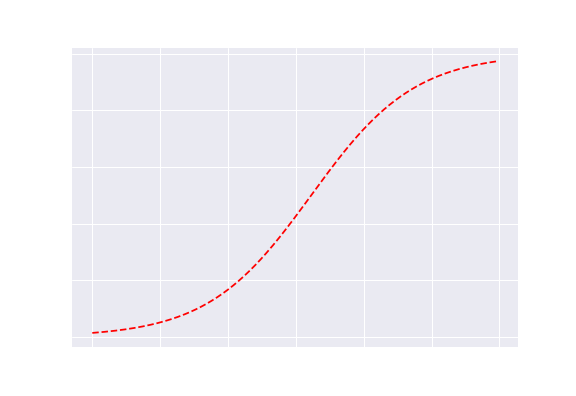
\includegraphics[scale=0.4]{graph_logistic.png}  
& 
\hspace{-30pt}
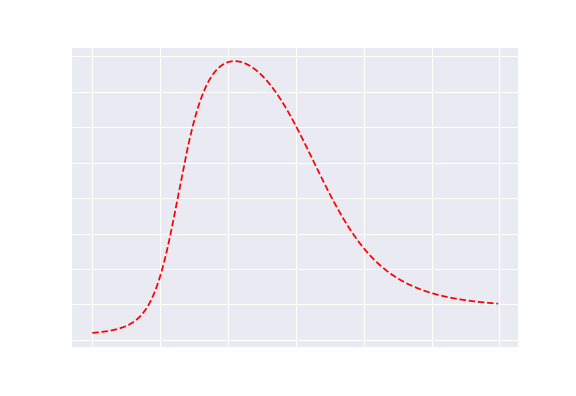
\includegraphics[scale=0.4]{graph_nn.png}  
\end{tabular}
}


\end{document}